% Provenance (never printed): see sources/outline_sources.md (Year 2: palaeogeography through
% the Phanerozoic; sea level; orogenies; mass extinctions and their Earth causes). Maps from the
% plate model of Merdith and others (2021) through the GPlates Web Service; sea level from the
% Miller and others (2005) NOAA study (Haq and others 1987; Kominz and others 2008); flooding and
% the Pitman model after Tasistro-Hart and Macdonald (2023); the big five after Marshall (2023)
% and Kaiho (2022); oceanic anoxic events after Rigo and others (2024) and Walker-Trivett and
% others (2024); CAMP carbon dioxide after Capriolo and others (2020); Chicxulub after
% Pickersgill and others (2026) and Collins and others (2020). Curves and numbers from
% figdata/bachelor-2/phanerozoic.py; exercise and problem values in the Book 4 scratch
% calculator calc/ch19.py.
\chapter{La Terre phanérozoïque}\label{ch:b2:phanerozoic-earth}

Dans l'ouest du Kansas, au cœur de l'Amérique du Nord, des piliers de craie blanche s'élèvent au-dessus
de la prairie. La craie est la vase d'un fond marin~: il y a environ 80 millions d'années, une mer peu
profonde traversait le centre de l'Amérique du Nord du nord au sud, et les coquilles d'algues flottantes
s'y déposaient au fond à quelques centièmes de millimètre par an. Cinq fois au cours des 540 derniers
millions d'années, une large part des espèces qui peuplaient ces mers a disparu en un instant géologique.
Ces deux histoires sont celles de la Terre elle-même~: les continents se sont déplacés, la mer s'est
élevée et retirée au-dessus d'eux, et au moins trois des cinq grandes extinctions ont coïncidé avec des
épanchements de lave venus de l'intérieur de la planète. Ce chapitre parcourt le Phanérozoïque à travers
ses cartes, son niveau marin, ses chaînes de montagnes et ses crises, et chiffre deux de ces crises~:
la vitesse à laquelle les dorsales élèvent la mer, et la surface de terre que noie une mer plus haute.
% ledger: kgs:monument-rocks, kgs:chalk, ics:base.Phanerozoic, kaiho22:table, cr03:table

\begin{recall}
\textbf{Des volumes scolaires}~: la tectonique des plaques et la Pangée~; les fossiles et l'échelle des temps
géologiques~; les transgressions lues dans une falaise. \textbf{Du volume de première année}~: la loi
profondeur--âge du plancher océanique~; la courbe hypsométrique~; l'isostasie~; l'eustatisme et le niveau relatif de
la mer~; les grandes provinces ignées~; les extinctions de masse comme marqueurs stratigraphiques, l'iridium
de la limite K--Pg et la datation de la crise de la fin du Permien~; les étages et les GSSP. \textbf{Des chapitres
précédents}~: les \omterm{def:b2:alpine-orogen:orogen}{orogènes} (\cref{ch:b2:alpine-orogen,ch:b2:himalaya-andes})~; le \omterm{def:b2:wilson-cycle:wilson}{cycle de Wilson} et les
\omterm{def:b2:wilson-cycle:supercontinent}{supercontinents} (\cref{ch:b2:wilson-cycle})~; le \omterm{def:b2:basins-compared:backstripping}{backstripping} (\cref{ch:b2:basins-compared})~; les boules de
neige du Cryogénien (\cref{ch:b2:precambrian-earth}). L'extinction et l'histoire du vivant relèvent des volumes
de biologie~; le volume de troisième année traite du paléomagnétisme et de la stratigraphie séquentielle.
\end{recall}

\section{Cartes d'un monde en mouvement}\label{sec:b2:phanerozoic-earth:maps}

Une roche se trouve rarement là où elle s'est formée. Un charbon, un grès désertique, un récif ont chacun
été déposés à une certaine latitude, puis emportés depuis par leur plaque. Avant que le climat ou la
vie d'une époque passée puisse être lu dans ces roches, il faut les replacer là où elles se trouvaient.

\begin{definition}[Paléogéographie~; carte paléogéographique]\label{def:b2:phanerozoic-earth:palaeogeography}
\emph{Paléogéographie}\index{paléogéographie} est la reconstruction de la géographie d'une
époque passée~: la position des continents et des océans, et de leurs rivages, chaînes de montagnes
et mers. Une \emph{carte paléogéographique}\index{carte paléogéographique} représente
cette géographie à un instant donné, sur la grille de latitude et de longitude de cette époque.
\end{definition}

Quatre sortes de preuves entrent dans une telle carte. L'aimantation des roches donne la latitude à laquelle
elles se sont formées, sujet du paléomagnétisme traité dans le volume de troisième année~; mais le champ
terrestre est symétrique par rapport à son axe, il ne dit donc rien de la longitude. Le plancher océanique
enregistre directement le mouvement des plaques, par ses bandes magnétiques et ses âges, mais seulement jusqu'au
plus ancien plancher conservé, vieux d'environ 190 millions d'années~: tout ce qui est plus ancien a
été subduit. Avant cela, l'ajustement des continents, les sutures et les \omterm{def:b2:alpine-orogen:orogen}{orogènes} là où les océans se sont
refermés, ainsi que les fossiles et les sédiments qui trahissent un climat --- récifs et évaporites sous les
tropiques, dépôts glaciaires près des pôles --- complètent le tableau. Les modèles de plaques rassemblent
ces contraintes et ramènent chaque plaque dans le passé~; les reconstructions doivent aussi tenir compte de
la lente rotation de toute la Terre solide par rapport à son axe de rotation, appelée dérive polaire vraie.
% ledger: vh26:palaeogeography, gws:merdith-frame, data:b2-seafloor-age, merdith21:model

\begin{omfigure}
\centering
% figdata/bachelor-2/phanerozoic.py parts map-<t>, cities-<t>, grat (Mollweide, x and y in Earth radii)
\begin{tikzpicture}
\begin{groupplot}[group style={group size=2 by 3, horizontal sep=0.35cm, vertical sep=0.55cm},
  width=0.53\linewidth, axis equal image, hide axis, clip=false,
  xmin=-2.85, xmax=2.85, ymin=-1.43, ymax=1.43,
  title style={font=\small, yshift=-1.5ex}]
\pgfplotsinvokeforeach{500,300,200,100,50,0}{
\nextgroupplot[title={#1~\unit{Ma}}]
\fill[omSea] (axis cs:0,0) ellipse [x radius=2.8284, y radius=1.4142];
\addplot[fill=omLithAlluv!85!black, draw=none] table[x=x, y=y]
  {figdata/out/bachelor-2-phanerozoic-map-#1.dat};
\addplot[black!35, line width=0.2pt] table[x=x, y=y] {figdata/out/bachelor-2-phanerozoic-grat.dat};
\draw[black!70, line width=0.4pt] (axis cs:0,0) ellipse [x radius=2.8284, y radius=1.4142];
\addplot[only marks, mark=*, mark size=1.3pt, red!75!black, point meta=explicit symbolic,
  nodes near coords, nodes near coords style={font=\tiny\bfseries, anchor=south west,
  inner sep=0.5pt, text=red!60!black}]
  table[x=x, y=y, meta=tag] {figdata/out/bachelor-2-phanerozoic-cities-#1.dat};
}
\end{groupplot}
\end{tikzpicture}
\par\smallskip{\small Les littoraux actuels ramenés à six époques dans le modèle de plaques de Merdith
et al. (2021), reconstruits par le GPlates Web Service, en projection de Mollweide à aires égales~;
parallèles tous les \ang{30}, méridiens tous les \ang{60}. Les points rouges suivent quatre villes~:
Paris (P), New York (N), Sydney (S) et Le Cap (C)~; à \qty{500}{Ma}, la croûte de Sydney n'est pas
encore présente dans le modèle. Les formes sont celles des littoraux actuels déplacés, et non celles
des rivages de ces époques~; dans ce référentiel paléomagnétique, les longitudes sont arbitraires.}
\end{omfigure}
% ledger: data:b4-palaeocoast, data:b4-palaeopos, geonames4:cities, gws:merdith-frame, merdith21:model

Les six cartes ci-dessus résument le Phanérozoïque. À \qty{500}{Ma}, les continents du Sud ne forment qu'une
seule masse, le Gondwana, en grande partie près du pôle Sud, avec la croûte de Paris à \ang{61}~S sur sa
marge. À \qty{300}{Ma}, les continents se sont réunis en Pangée, assemblée à partir d'environ \qty{325}{Ma}
et disloquée à partir d'environ \qty{200}{Ma}~: Paris et New York se trouvent sur l'équateur, Le Cap et
Sydney vers \ang{60}~S. À \qty{200}{Ma}, le \omterm{def:b2:wilson-cycle:supercontinent}{supercontinent} est complet, une terre unique qui s'étend des hautes
latitudes nord aux hautes latitudes sud~; à \qty{100}{Ma}, l'Atlantique et l'océan Indien se sont ouverts,
et à \qty{50}{Ma} la carte est presque celle d'aujourd'hui, l'Australie restant proche de l'Antarctique.
% ledger: data:b4-palaeopos, nance22:supercontinents

\begin{example}[Paris dérive vers le nord]\label{ex:b2:phanerozoic-earth:paris}
Dans le modèle, Paris se trouvait à \ang{5.1}~N il y a \qty{300}{Ma}~; il se trouve aujourd'hui
à \ang{48.9}~N. Sa latitude a donc augmenté de \ang{43.8}, soit $43.8 \times 111.2 = \qty{4871}{km}$
le long d'un méridien ($\qty{111.2}{km}$ par degré sur une sphère de rayon \qty{6371}{km}),
à une vitesse moyenne de $4871/300 = \qty{16}{km}$ par million d'années, soit \qty{1.6}{cm}
par an. Ce n'est que la part nord du déplacement~: le référentiel paléomagnétique laisse la
longitude libre, de sorte que la distance réellement parcourue était au moins égale à celle-ci.
\end{example}
% ledger: data:b4-palaeopos, geonames4:cities, earth:Rmean, gws:merdith-frame
% values: calc/ch19.py (43.8 deg, 4870.6 km, 16.2 km/Myr)

\section{Le niveau de la mer au cours du Phanérozoïque}\label{sec:b2:phanerozoic-earth:sealevel}

\subsection*{Mers sur les continents}

Pendant l'essentiel du Phanérozoïque, une bien plus grande part des continents était sous la
mer qu'aujourd'hui. Les roches marines d'Amérique du Nord gardent la trace de plusieurs submersions
de l'intérieur du continent, la première étant la transgression cambrienne qui scelle la
Grande Discordance~; à la fin du Crétacé, d'environ 120 à \qty{80}{Ma}, des sédiments marins
se sont accumulés à travers l'Ouest intérieur, au cœur du continent (photographie ci-dessous).
% ledger: th23:flooding, th23:wib

\begin{omfigure}
\centering
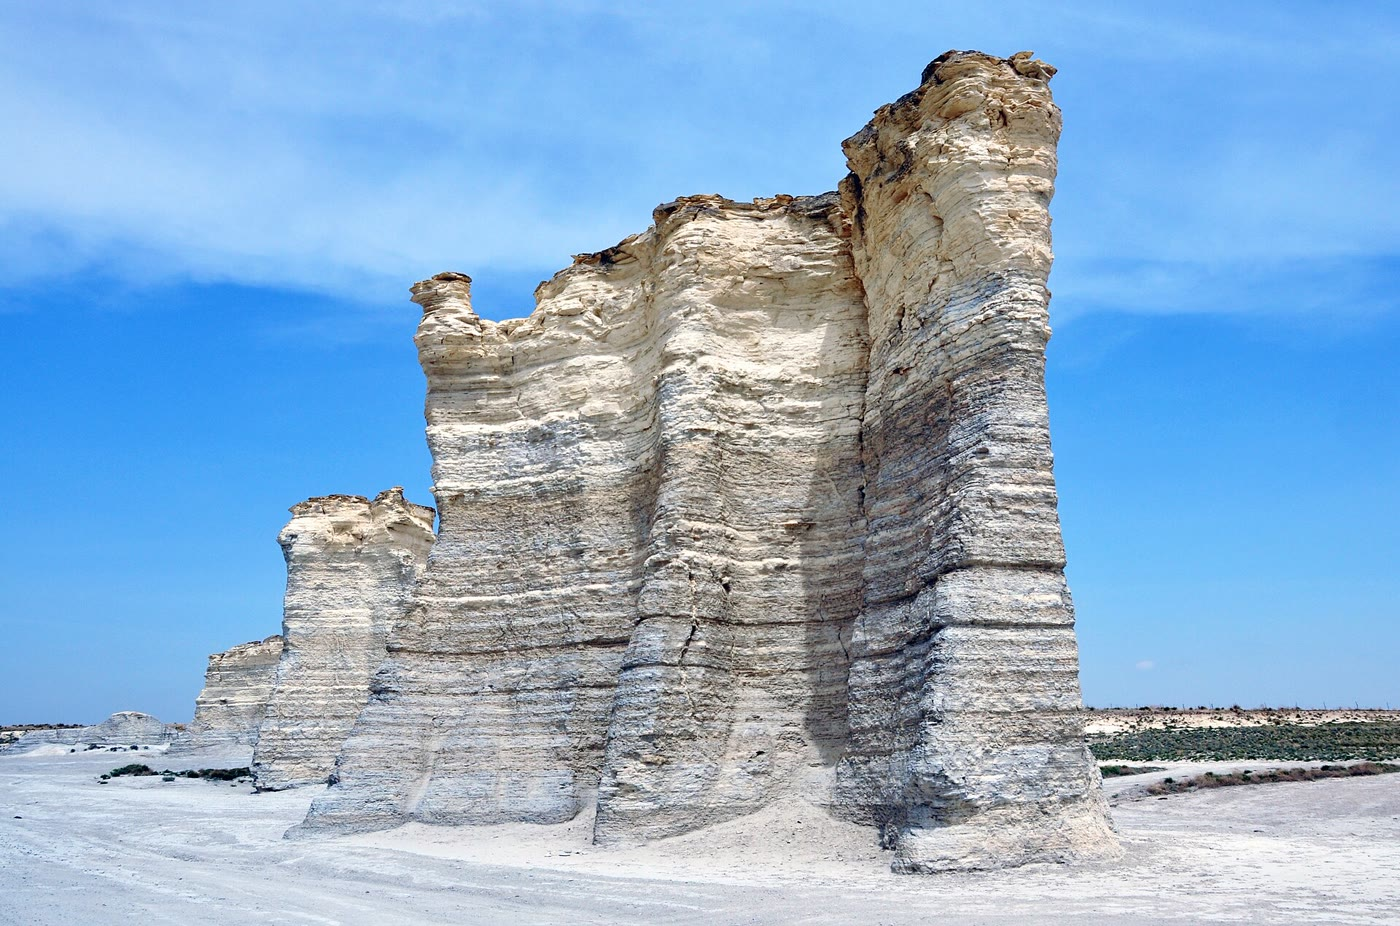
\includegraphics[width=0.66\linewidth]{images/book4/b2-19-monument-rocks.jpg}
\par\smallskip{\small Monument Rocks, Kansas occidental~: piliers de craie, vase
d'une mer intérieure du Crétacé vieille d'environ 80 millions d'années, déposée à
environ \qty{0.036}{mm} par an. (James St.~John, CC~BY~2.0, via Wikimedia Commons.)}
\end{omfigure}
% ledger: kgs:monument-rocks, kgs:chalk

\begin{definition}[Mer épicontinentale]\label{def:b2:phanerozoic-earth:epeiric}
Une \emph{mer épicontinentale}\index{mer épicontinentale} est une mer peu profonde qui recouvre
l'intérieur d'un continent, sur la croûte continentale, loin de la marge continentale.
\end{definition}

La mer atteint de tels intérieurs en déplaçant son rivage, et les roches en gardent la trace.

\begin{definition}[Transgression marine~; régression marine]\label{def:b2:phanerozoic-earth:transgression}
Une \emph{transgression marine}\index{transgression marine} est un déplacement vers l'intérieur
des terres du rivage, par lequel la mer envahit la terre~; une
\emph{régression marine}\index{régression marine} est un déplacement vers le large, par lequel la terre émerge.
\end{definition}

Dans une coupe verticale, une transgression superpose des dépôts de plus grande profondeur à des
dépôts moins profonds --- des vases du large sur des sables de plage --- et une régression fait
l'inverse. Les deux suivent le niveau relatif de la mer, qui mêle le niveau marin global à
l'affaissement ou au soulèvement du lieu et à l'apport de sédiments~: un delta peut faire avancer
son rivage vers le large alors que la mer monte, s'il est alimenté assez vite. Pour lire le niveau
marin global dans les transgressions, un géologue doit retrouver le même signal sur plusieurs
continents, ou retirer l'affaissement par \omterm{def:b2:basins-compared:backstripping}{backstripping}, comme au \cref{ch:b2:basins-compared}.
% ledger: miller20:rsl

\subsection*{La courbe à long terme}

\begin{definition}[Cycle eustatique de premier ordre]\label{def:b2:phanerozoic-earth:first-order}
Le \emph{cycle eustatique de premier ordre}\index{cycle eustatique de premier ordre} est la partie
la plus lente de la variation du niveau marin global, sur des échelles de dizaines à centaines
de millions d'années, fixée par la tectonique de la Terre solide plutôt que par les glaces.
\end{definition}

Sur l'ensemble du Phanérozoïque, la courbe de premier ordre a la forme d'un M~: haute au Paléozoïque
inférieur, basse pendant que la Pangée s'assemblait et subsistait, du Carbonifère à la fin du Trias, de
nouveau haute au Crétacé, puis en baisse depuis. Extrapolée à partir de l'Amérique du Nord, la
submersion de la fin de l'Ordovicien suggère à elle seule une hausse supplémentaire de 100 à \qty{200}{m}.
Des variations plus rapides se superposent à cette courbe~: celles dues aux glaces
s'enregistrent sur des échelles de temps de $10^4$ à $10^6$ ans, et la calotte
antarctique, depuis environ \qty{33.5}{Ma}, a déplacé la mer de 50 à \qty{60}{m}.
% ledger: th23:flooding, miller11:greenhouse, miller05:abstract

\begin{omfigure}
\centering
% figdata/bachelor-2/phanerozoic.py parts sealevel-haq, sealevel-haqlt, sealevel-kominz, sealevel-kominzlt
\begin{tikzpicture}
\begin{axis}[width=0.92\linewidth, height=6.2cm, x dir=reverse, xmin=0, xmax=252,
  ymin=-130, ymax=280, xlabel={âge (\unit{Ma})}, ylabel={niveau de la mer au-dessus d'aujourd'hui (\unit{m})},
  xtick={0,50,...,250}, ytick={-100,-50,...,250}, xtick pos=bottom, ytick pos=left,
  tick label style={font=\scriptsize}, label style={font=\small},
  legend style={at={(0.5,1.04)}, anchor=south, draw=none, font=\scriptsize, legend columns=2,
  /tikz/every even column/.append style={column sep=8pt}}]
\addplot[black!30, line width=0.3pt] table[x=age_ma, y=sl_m]
  {figdata/out/bachelor-2-phanerozoic-sealevel-haq.dat};
\addlegendentry{Haq et al. (1987)}
\addplot[omThm, line width=0.3pt] table[x=age_ma, y=sl_m]
  {figdata/out/bachelor-2-phanerozoic-sealevel-kominz.dat};
\addlegendentry{New Jersey, backstripping}
\addplot[black, line width=1.2pt] table[x=age_ma, y=sl_m]
  {figdata/out/bachelor-2-phanerozoic-sealevel-haqlt.dat};
\addlegendentry{Haq, moyenne sur 10 Ma}
\addplot[omThm!70!black, line width=1.2pt] table[x=age_ma, y=sl_m]
  {figdata/out/bachelor-2-phanerozoic-sealevel-kominzlt.dat};
\addlegendentry{New Jersey, moyenne sur 10 Ma}
\addplot[black!50, line width=0.3pt, forget plot] coordinates {(0,0) (252,0)};
\foreach \a/\b/\c in {251.902/201.4/icsTriassic, 201.4/143.1/icsJurassic,
  143.1/66/icsCretaceous, 66/23.04/icsPaleogene, 23.04/2.58/icsNeogene, 2.58/0/icsQuaternary} {
  \edef\tmp{\noexpand\fill[\c] (axis cs:\a,-130) rectangle (axis cs:\b,-112);}\tmp}
\node[font=\tiny, text=white] at (axis cs:226.7,-121) {Trias};
\node[font=\tiny, text=white] at (axis cs:172.3,-121) {Jurassique};
\node[font=\tiny] at (axis cs:104.6,-121) {Crétacé};
\node[font=\tiny] at (axis cs:44.5,-121) {Paléogène};
\node[font=\tiny] at (axis cs:12.8,-121) {Néog.};
\end{axis}
\end{tikzpicture}
\par\smallskip{\small Niveau marin global depuis \qty{250}{Ma}, tel que tabulé par Miller et al. (2005)~:
la courbe des cycles de Haq et al. (1987), établie à partir de la stratigraphie de nombreux bassins, et le
niveau marin corrigé de l'affaissement (\omterm{def:b2:basins-compared:backstripping}{backstripping}) à partir de sondages de New Jersey, avec les bas
niveaux estimés (Kominz et al. 2008). Traits épais~: moyennes glissantes sur 10 Ma, soit la tendance de
premier ordre. Les âges sont donnés sur l'échelle de temps de 2012~; la bande du bas indique les périodes.}
\end{omfigure}
% ledger: data:b4-sealevel, haq87:charts, kominz08:long-term, ics:base.Triassic, ics:base.Jurassic, ics:base.Cretaceous, ics:base.Paleogene, ics:base.Neogene, ics:base.Quaternary, ics:colour.Triassic, ics:colour.Jurassic, ics:colour.Cretaceous, ics:colour.Paleogene, ics:colour.Neogene, ics:colour.Quaternary

Les deux courbes ci-dessus s'accordent sur la forme et divergent sur l'amplitude. La courbe des cycles,
construite à partir de l'empilement des sédiments de nombreux bassins, place le niveau marin à long terme
du milieu du Crétacé à environ \qty{233}{m} au-dessus d'aujourd'hui~; les sondages de New Jersey, corrigés
un par un de l'affaissement, donnent environ \qty{70}{m} au Crétacé supérieur et un maximum voisin de
\qty{110}{m} à l'Éocène. Miller et ses collègues concluent que le maximum à long terme du Crétacé était de
$100 \pm \qty{50}{m}$, et que les courbes des cycles, justes quant à la date des baisses, exagèrent leurs
amplitudes. New Jersey n'est pas non plus une jauge parfaite~: sa mer du Crétacé supérieur est de 100 à
\qty{150}{m} plus basse que ne le prédit le volume des bassins océaniques, un écart que pourrait expliquer
l'affaissement de la région au-dessus de la plaque de Farallon subduite --- la topographie dynamique.
% ledger: data:b4-sealevel, miller05:abstract, kominz08:long-term, miller20:epr

\subsection*{Pourquoi la mer se déplace~: les dorsales}

Qu'est-ce qui élève la mer de cent mètres pendant des dizaines de millions d'années~? Pas les
glaces~: le Crétacé était un monde chaud, avec tout au plus de petites calottes brèves. La
réponse principale est le volume des dorsales océaniques. Un plancher océanique jeune est
chaud et se tient haut~; plus les plaques s'écartent vite, plus le plancher est jeune en
moyenne, moins les bassins océaniques sont profonds, et plus l'eau déborde sur les continents.
% ledger: miller11:greenhouse, th23:pitman

\begin{proposition}[Niveau de la mer et vitesse d'expansion]\label{prop:b2:phanerozoic-earth:ridge}
Soit un plancher océanique d'aire $A_{\text{f}}$ créé aux dorsales de longueur totale $L$ à la
vitesse d'expansion complète $u$, et détruit à l'âge $\tau = A_{\text{f}}/(Lu)$, chaque âge entre
0 et $\tau$ couvrant la même aire. Soit $d(t) = d_{\text{r}} + c\sqrt t$ la loi de profondeur.
\begin{enumerate}
  \item La profondeur moyenne du plancher est $\bar d = d_{\text{r}} + \tfrac23 c\sqrt\tau$.
  \item Si la vitesse d'expansion devient $fu$, avec $A_{\text{f}}$ et $L$ inchangés, la profondeur moyenne diminue de
        $\Delta\bar d = \tfrac23 c\sqrt\tau\,\bigl(1 - f^{-1/2}\bigr)$.
  \item Si le plancher s'enfonce isostatiquement sous l'eau ajoutée, et si la mer ne submerge pas les terres,
        le niveau de la mer au-dessus d'un océan d'aire $A_{\text{o}}$ s'élève de
        \[
        \Delta s = \frac{\rho_{\text{m}} - \rho_{\text{w}}}{\rho_{\text{m}}}\,
        \frac{A_{\text{f}}}{A_{\text{o}}}\,\Delta\bar d ,
        \]
        avec $\rho_{\text{m}}$ la masse volumique du manteau et $\rho_{\text{w}}$ celle de l'eau de mer.
\end{enumerate}
\end{proposition}

\begin{proof}
(1) Les dorsales créent du plancher neuf au rythme $Lu$ (aire par unité de temps), et chaque bande de plancher vit pendant
le temps $\tau$~; en régime permanent, l'aire du plancher d'âge compris entre $t$ et $t + \mathrm{d}t$
vaut $Lu\,\mathrm{d}t$ pour tout $t < \tau$, donc l'aire totale vaut $Lu\tau = A_{\text{f}}$ et les âges sont
également répartis. La profondeur moyenne vaut
$\frac1\tau\int_0^\tau (d_{\text{r}} + c\sqrt t)\,\mathrm{d}t = d_{\text{r}} + \frac{c}{\tau}
\cdot\frac23\tau^{3/2}$. (2) Avec la vitesse $fu$, $\tau$ devient $\tau/f$, et
$\sqrt{\tau/f} = f^{-1/2}\sqrt\tau$. (3) Les bassins perdent le volume $\Delta V = A_{\text{f}}
\Delta\bar d$. Soit $\Delta s$ la hausse de la surface de la mer par rapport aux continents, et $y$ l'affaissement du plancher
sous l'eau supplémentaire. La colonne d'eau supplémentaire, d'épaisseur $\Delta s + y$, remplace une
épaisseur $y$ de manteau dans l'équilibre isostatique~: $\rho_{\text{w}}(\Delta s + y) =
\rho_{\text{m}} y$, donc $y = \rho_{\text{w}}\Delta s/(\rho_{\text{m}} - \rho_{\text{w}})$ et
$\Delta s + y = \Delta s\,\rho_{\text{m}}/(\rho_{\text{m}} - \rho_{\text{w}})$. Le volume se conserve~:
$A_{\text{o}}(\Delta s + y) = \Delta V$, ce qui donne le résultat.
\end{proof}

Le plancher réel n'est pas si ordonné. Ses âges ne sont pas répartis également~: le plancher jeune
est le plus abondant, et son aire décroît avec l'âge, comme le montre le panneau de gauche ci-dessous.
La loi en racine carrée ne tient pas davantage pour le plancher ancien, qui s'aplatit vers
\qty{6.4}{km}~; la loi exponentielle que Parsons et Sclater ont ajustée au plancher ancien, la loi de
plaque, prend le relais au-delà d'environ \qty{26}{Ma}, là où les deux lois se rejoignent. La proposition
n'est qu'une première estimation, et la figure montre à quel point la seconde loi la modifie.
% ledger: ps77:depth-age, data:b4-ridge

\begin{omfigure}
\centering
% figdata/bachelor-2/phanerozoic.py parts agehist and ridge
\begin{tikzpicture}
\begin{groupplot}[group style={group size=2 by 1, horizontal sep=1.6cm},
  width=0.5\linewidth, height=5.6cm, tick label style={font=\scriptsize},
  label style={font=\small}, xtick pos=bottom, ytick pos=left]
\nextgroupplot[xmin=0, xmax=200, ymin=0, ymax=34, xlabel={âge du plancher (\unit{Ma})},
  ylabel={aire par tranche de \qty{10}{Ma} (\unit{\mega km^2})},
  legend style={at={(0.5,1.04)}, anchor=south, draw=none, font=\scriptsize}]
\addplot[ybar interval, area legend, fill=omSea!80!black, draw=black!50, line width=0.2pt]
  table[x expr=\thisrow{age}-5, y=area_Mkm2] {figdata/out/bachelor-2-phanerozoic-agehist.dat};
\addlegendentry{grille des âges}
\addplot[const plot mark mid, black, dashed, line width=0.9pt]
  table[x=age, y=uniform_Mkm2] {figdata/out/bachelor-2-phanerozoic-agehist.dat};
\addlegendentry{âges répartis jusqu'à \qty{128.4}{Ma}}
\nextgroupplot[xmin=1, xmax=3, ymin=0, ymax=650, xlabel={vitesse d'expansion / actuelle, $f$},
  ylabel={hausse du niveau de la mer $\Delta s$ (\unit{m})},
  legend style={at={(0.5,1.04)}, anchor=south, draw=none, font=\scriptsize, legend columns=2}]
\fill[omThm!15] (axis cs:1,50) rectangle (axis cs:3,150);
\addplot[black, line width=1pt] table[x=f, y=ds_hs] {figdata/out/bachelor-2-phanerozoic-ridge.dat};
\addlegendentry{loi en $\sqrt t$}
\addplot[blue!70!black, dashed, line width=1pt] table[x=f, y=ds_plate]
  {figdata/out/bachelor-2-phanerozoic-ridge.dat};
\addlegendentry{loi de plaque}
\node[font=\scriptsize, anchor=west] at (axis cs:1.6,100) {$100 \pm \qty{50}{m}$};
\end{groupplot}
\end{tikzpicture}
\par\smallskip{\small À gauche~: aire du plancher océanique actuel en classes d'âge de 10 Ma, d'après la
grille des âges de Seton et al. (2020) à un degré de résolution (\qty{293}{\mega km^2} au total), comparée
à la répartition uniforme de la \cref{prop:b2:phanerozoic-earth:ridge}, de même aire et même âge moyen. À
droite~: hausse du niveau de la mer lorsque la vitesse d'expansion est multipliée par $f$, d'après la
proposition avec la loi en racine carrée et avec la loi de plaque, à partir de la répartition uniforme jusqu'à
\qty{128.4}{Ma}~; la bande est le maximum à long terme du Crétacé estimé par Miller et al. (2005).}
\end{omfigure}
% ledger: data:b4-ridge, data:b2-seafloor-age, seton:mean-age, ps77:depth-age, miller05:abstract, charette:ocean-volume, katz03:thermo, noaa:seawater-1025

\begin{example}[Deux fois plus vite]\label{ex:b2:phanerozoic-earth:doubling}
Prenons le plancher d'aujourd'hui~: âge moyen \qty{64.2}{Ma}, donc $\tau = \qty{128.4}{Ma}$ dans le modèle réparti~;
$d_{\text{r}} = \qty{2500}{m}$, $c = \qty{350}{m.Ma^{-1/2}}$. La profondeur moyenne vaut $2500 + \tfrac23
\times 350 \times \sqrt{128.4} = \qty{5144}{m}$. Doubler la vitesse divise $\tau$ par deux, et la profondeur
moyenne devient $2500 + \tfrac23 \times 350 \times \sqrt{64.2} = \qty{4370}{m}$~: le plancher remonte en moyenne
de \qty{774}{m}. Avec $A_{\text{f}}/A_{\text{o}} = 293/362 = 0.8094$ et
$(\rho_{\text{m}} - \rho_{\text{w}})/\rho_{\text{m}} = (3300 - 1025)/3300 = 0.689$, la mer monte de
$0.689 \times 0.8094 \times 774 = \qty{432}{m}$~; avec la loi de plaque, \qty{368}{m}. Ce sont deux valeurs
environ quatre fois supérieures au maximum à long terme du Crétacé. Lue à l'envers, le panneau de droite dit
qu'une vitesse d'expansion seulement 15 à \qty{20}{\percent} supérieure à celle d'aujourd'hui suffit pour \qty{100}{m}, ce qui
conduit Miller et ses collègues à conclure que la croûte océanique a été produite beaucoup plus lentement
au Crétacé qu'on ne l'avait supposé.
\end{example}
% ledger: seton:mean-age, ps77:depth-age, data:b4-ridge, charette:ocean-volume, katz03:thermo, noaa:seawater-1025, miller05:abstract
% values (phanerozoic.py numbers): dbar_hs 5144, dbar_hs_half 4369.6, rise2_hs 432.5, rise2_pl 368.4, f_for_100_hs 1.151

Le modèle est aussi trop profond~: sa profondeur moyenne, \qty{5144}{m}, dépasse la profondeur moyenne mesurée du
plancher daté, \qty{4265}{m}, en partie parce que la loi en racine carrée surestime le plancher ancien, et en
partie parce que le plancher réel porte des sédiments, des \omterm{def:b2:oceanic-islands:seamount}{monts sous-marins} et des plateaux que la loi ignore.
Et la vitesse d'expansion n'est pas le seul levier. Les dorsales sont compensées par les fosses~: si le plancher
océanique s'élève en un endroit, la masse doit aller ailleurs, et un continent qui s'enfonce au-dessus d'une
plaque plongeante --- la topographie dynamique --- laisse localement entrer la mer. Tasistro-Hart et Macdonald
soutiennent que les submersions de l'Amérique du Nord suivent les plaques plongeant sous le continent, et que le
niveau marin global dépend de la part de subduction qui se produit sous les continents plutôt que sous les océans.
% ledger: data:b4-floor-depth, th23:pitman, th23:flooding, kominz08:long-term

\section{Submersion des continents}\label{sec:b2:phanerozoic-earth:flooding}

La surface de terre qu'une hausse de la mer submerge dépend de la forme de la surface terrestre, que
résume la courbe hypsométrique du volume de première année~: la fraction de la surface qui s'élève
au-dessus de chaque altitude (figure ci-dessous, à gauche). Les continents ont un sommet plat. Sur
la grille d'ETOPO1 à un degré, \qty{29.0}{\percent} de la surface est émergée et \qty{34.3}{\percent}
s'élève au-dessus de \qty{-200}{m}~: les plateaux continentaux, déjà sous l'eau, font la différence.
La plus grande part des terres est basse, si bien qu'une hausse modeste en submerge beaucoup.
% ledger: data:b4-hyps, data:etopo1

\begin{proposition}[Submersion des terres]\label{prop:b2:phanerozoic-earth:flooding}
Soit $A_{\text{o}}$ l'aire de la mer aujourd'hui et $a(z)$ l'aire des
terres plus basses que $z$ au-dessus du niveau actuel de la mer. Un volume
$V$ d'eau ajouté à la mer élève son niveau de la hauteur $s$ qui vérifie
\[
V = \int_0^s \bigl(A_{\text{o}} + a(z)\bigr)\,\mathrm{d}z ,
\]
et submerge l'aire de terre $a(s)$. Comme $a \ge 0$, la hausse est au plus égale à $V/A_{\text{o}}$.
\end{proposition}

\begin{proof}
Lorsque la mer se tient à $z$, elle couvre $A_{\text{o}} + a(z)$~; la relever de $\mathrm{d}z$
demande le volume $\bigl(A_{\text{o}} + a(z)\bigr)\mathrm{d}z$. En sommant de 0 à $s$, on
obtient $V$. L'intégrande est au moins égale à $A_{\text{o}}$, donc $V \ge A_{\text{o}}s$.
\end{proof}

\begin{omfigure}
\centering
% figdata/bachelor-2/phanerozoic.py parts hyps and flood
\begin{tikzpicture}
\begin{groupplot}[group style={group size=2 by 1, horizontal sep=1.6cm},
  width=0.46\linewidth, height=5.6cm, tick label style={font=\scriptsize},
  label style={font=\small}, xtick pos=bottom, ytick pos=left]
\nextgroupplot[xmin=0, xmax=100, ymin=-9500, ymax=6500,
  xlabel={pourcentage de la surface au-dessus de $z$}, ylabel={altitude $z$ (\unit{m})},
  scaled y ticks=false, yticklabel style={/pgf/number format/1000 sep={\,}}]
\addplot[omThm, line width=1pt] table[x=pct, y=z] {figdata/out/bachelor-2-phanerozoic-hyps.dat};
\addplot[black!50, line width=0.3pt] coordinates {(0,0) (100,0)};
\node[font=\scriptsize, anchor=south west] at (axis cs:30,100) {terres \qty{29.0}{\percent}};
\node[font=\scriptsize] at (axis cs:45,-7000) {plancher océanique};
\nextgroupplot[xmin=0, xmax=1000, ymin=0, ymax=80, xlabel={hausse du niveau de la mer $h$ (\unit{m})},
  ylabel={terres submergées (\unit{\percent})}]
\addplot[omThm, line width=1pt] table[x=h, y=flooded_pct]
  {figdata/out/bachelor-2-phanerozoic-flood.dat};
\addplot[black, dashed, line width=0.5pt] coordinates {(100,0) (100,14.9) (0,14.9)};
\addplot[black, dashed, line width=0.5pt] coordinates {(432,0) (432,50.6) (0,50.6)};
\end{groupplot}
\end{tikzpicture}
\par\smallskip{\small À gauche~: courbe hypsométrique de la Terre, à partir de la grille ETOPO1 à un degré. À droite~:
pourcentage des terres actuelles situées sous chaque hauteur au-dessus du niveau de la mer, soit les terres
qu'une hausse $h$ submergerait si rien d'autre ne bougeait~; les tirets marquent \qty{100}{m} et \qty{432}{m}. La
moyenne sur des cellules d'un degré lisse le relief, de sorte que ces valeurs ne sont que des premières estimations.}
\end{omfigure}
% ledger: data:b4-hyps, data:etopo1

Le panneau de droite donne la réponse d'emblée. Une hausse de \qty{100}{m} submerge environ \qty{15}{\percent}
des terres actuelles~; les \qty{432}{m} d'une vitesse d'expansion doublée en submergeraient la moitié.
Une telle mer s'étend sur les terres qu'elle submerge, de sorte que la hausse elle-même est inférieure
à la borne $V/A_{\text{o}}$ de la proposition, d'environ un dixième pour une hausse de quelques centaines
de mètres (problème du week-end). Les mers du Crétacé du Kansas avaient besoin de beaucoup moins~:
l'intérieur d'un continent est souvent bas, et il peut aussi s'enfoncer au-dessus d'une plaque plongeante.
% ledger: data:b4-hyps
% values (phanerozoic.py numbers): flood_100 14.9, flood_rise2 50.8, level_rise2_spread 390.7

\section{Chaînes de montagnes du Phanérozoïque}\label{sec:b2:phanerozoic-earth:orogens}

Chaque \omterm{def:b2:wilson-cycle:wilson}{cycle de Wilson} décrit au \cref{ch:b2:wilson-cycle} se termine par une chaîne de montagnes, et les chaînes phanérozoïques
marquent la formation puis la fragmentation de la Pangée. Le tableau rassemble celles qui sont abordées dans ce volume.

\begin{center}
\small
\begin{tabular}{>{\raggedright\arraybackslash}p{0.15\linewidth}>{\raggedright\arraybackslash}p{0.22\linewidth}>{\raggedright\arraybackslash}p{0.22\linewidth}>{\raggedright\arraybackslash}p{0.29\linewidth}}
\hline
orogenèse & époque & océan refermé & ce qui s'est rencontré \\
\hline
Calédonien & vers~540--400 Ma~; collision principale 425--400 Ma & Iapetus & Laurentia, Baltica et
Avalonia, formant Laurussia \\
Varisque--appalachien & depuis vers~550 Ma~; collision finale Carbonifère supérieur--Permien & Rhéique &
le Gondwana et ses \omterm{def:b2:wilson-cycle:terrane}{terranes} détachées avec Laurussia, formant la Pangée \\
Alpin & Crétacé (maximum vers 100 Ma) et Cénozoïque & Téthys alpine & Apulie et Europe \\
Himalayen & depuis vers 60 à 54 Ma (débattu) jusqu'à aujourd'hui & océan au nord de l'Inde & Inde et Asie \\
Andin & toujours actif~; raccourcissement depuis l'Oligocène & aucun océan~: une plaque océanique plonge & la
plaque de Nazca sous l'Amérique du Sud \\
\hline
\end{tabular}
\end{center}
% ledger: mckerrow00:caledonian, schiffer20:caledonides, schiffer20:variscan, faure24:variscan, usgs:alleghanian-age, schmid04:two-orogenies, najman21:collision-age, gerbault05:andes, nance22:supercontinents

Les deux premières chaînes ont cousu la Pangée ensemble, la Varisque refermant le dernier
océan entre le Gondwana et Laurussia~; les trois dernières se sont formées tandis que les
morceaux de la Pangée s'écartaient et que les océans qui les séparaient étaient consumés. Le
bas niveau marin du Paléozoïque supérieur et du Trias appartient à ce \omterm{def:b2:wilson-cycle:supercontinent}{supercontinent}, et
la mer haute du Crétacé à sa dislocation, avec de nouvelles dorsales et un plancher jeune.
% ledger: schiffer20:variscan, th23:flooding, nance22:supercontinents

\section{Crises du vivant}\label{sec:b2:phanerozoic-earth:extinctions}

\subsection*{Les big five}

Les volumes de biologie décrivent les extinctions de masse~; les géologues les mesurent dans les
roches et en cherchent les causes. Cinq se détachent dans la chronique des animaux marins, les
«~big five~»~: à la fin de l'Ordovicien, vers \qty{444}{Ma}~; au Dévonien supérieur, \qty{372}{Ma}~;
à la fin du Permien, \qty{251.9}{Ma}~; à la fin du Trias, \qty{201.4}{Ma}~; et à la fin du
Crétacé, \qty{66}{Ma}. Chacune a éliminé entre environ deux cinquièmes et deux tiers des genres
d'animaux marins de la compilation de Sepkoski. La crise de la fin du Permien fut la plus grande~:
\qty{56}{\percent} des genres à la résolution la plus fine, et environ \qty{81}{\percent} des espèces
marines --- et non les \qty{96}{\percent} souvent cités, qui mêlaient deux crises distinctes.
% ledger: kaiho22:table, marshall23:big-five, stanley16:permian

\begin{history}[Les «~big five~», quarante ans après]
En 1982, D.~M.~Raup et J.~J.~Sepkoski dénombrèrent les familles d'animaux marins qui disparurent dans
chacun des 76 étages du Phanérozoïque. Quatre points dépassèrent la limite de confiance à 99~pour~cent
de leur tendance --- le dernier étage de l'Ordovicien, les deux derniers du Permien et le dernier du
Crétacé --- et la fin du Trias comme la fin du Dévonien dépassèrent la limite de 95~pour~cent~: ce
sont les big five. Quarante ans plus tard, les cinq restent les plus grandes crises depuis le début de
l'Ordovicien, mais, avec de meilleures données, elles ne se détachent plus d'un continuum de taux
d'extinction, et certains intervalles du Cambrien présentèrent des taux encore plus élevés. La résolution
temporelle de Raup et Sepkoski était de \qty{7.4}{Ma}, la durée moyenne d'un étage à l'époque~;
certaines crises furent brutales, d'autres durèrent des centaines de milliers d'années, voire davantage.
\end{history}
% ledger: marshall23:big-five, marshall23:resolution

\begin{omfigure}
\centering
% figdata/bachelor-2/phanerozoic.py parts ext, lip, oae
\begin{tikzpicture}
\begin{axis}[width=0.95\linewidth, height=6.4cm, x dir=reverse, xmin=0, xmax=541,
  ymin=-34, ymax=80, xlabel={âge (\unit{Ma})}, ylabel={genres marins perdus (\unit{\percent})},
  xtick={0,100,...,500}, ytick={0,20,...,80}, xtick pos=bottom, ytick pos=left,
  tick label style={font=\scriptsize}, label style={font=\small}, clip=false]
\addplot[ybar, bar width=5pt, fill=omThm!70, draw=black!60]
  % étiquettes : nœuds explicites (la table figdata porte les noms anglais)
  table[x=age, y=value] {figdata/out/bachelor-2-phanerozoic-ext.dat}; \foreach \a/\v/\t in {444/52/fin de l'Ordovicien, 372/41/Dévonien supérieur, 251.9/66/fin du Permien, 201.4/46/fin du Trias, 66/45/fin du Crétacé} {\edef\temp{\noexpand\node[font=\noexpand\tiny, anchor=south] at (axis cs:\a,\v) {\t};}\temp}
\addplot[only marks, mark=triangle*, mark size=2.6pt, red!70!black]
  table[x=age, y expr=-6] {figdata/out/bachelor-2-phanerozoic-lip.dat};
\addplot[only marks, mark=diamond*, mark size=2.6pt, blue!70!black]
  table[x=age, y expr=-13] {figdata/out/bachelor-2-phanerozoic-oae.dat};
\addplot[only marks, mark=star, mark size=4pt, line width=1pt, black] coordinates {(66,-20)};
\node[font=\tiny, anchor=west, red!70!black] at (axis cs:541,-6) {GPI};
\node[font=\tiny, anchor=west, blue!70!black] at (axis cs:541,-13) {EAO};
\node[font=\tiny, anchor=west] at (axis cs:541,-20) {impact};
\node[font=\tiny, anchor=west] at (axis cs:57,-20) {Chicxulub};
\foreach \a/\b/\c in {538.8/486.85/icsCambrian, 486.85/443.1/icsOrdovician,
  443.1/419.62/icsSilurian, 419.62/358.86/icsDevonian, 358.86/298.9/icsCarboniferous,
  298.9/251.902/icsPermian, 251.902/201.4/icsTriassic, 201.4/143.1/icsJurassic,
  143.1/66/icsCretaceous, 66/23.04/icsPaleogene, 23.04/2.58/icsNeogene, 2.58/0/icsQuaternary} {
  \edef\tmp{\noexpand\fill[\c] (axis cs:\a,-34) rectangle (axis cs:\b,-27);}\tmp}
\foreach \x/\t in {512.8/Cm, 465/O, 431.4/S, 389.2/D, 328.9/C, 275.4/P, 226.7/T, 172.3/J,
  104.6/Cr, 44.5/Pg, 12.8/N} {
  \edef\tmp{\noexpand\node[font=\noexpand\tiny] at (axis cs:\x,-30.5) {\t};}\tmp}
\end{axis}
\end{tikzpicture}
\par\smallskip{\small Les big five, avec la part des genres marins perdus dans la compilation
de Sepkoski (Kaiho 2022, tableau~1), les grandes provinces ignées (triangles, âges moyens de
Courtillot et Renne 2003, à partir de \qty{259}{Ma}), les \omterm{def:b2:phanerozoic-earth:oae}{événements anoxiques océaniques}
les mieux étudiés (losanges) et l'impact de Chicxulub. La barre du bas indique les périodes.}
\end{omfigure}
% ledger: kaiho22:table, cr03:table, rigo24:oaes, pickersgill26:chicxulub, ics:base.Cambrian, ics:base.Ordovician, ics:base.Silurian, ics:base.Devonian, ics:base.Carboniferous, ics:base.Permian, ics:base.Triassic, ics:base.Jurassic, ics:base.Cretaceous, ics:base.Paleogene, ics:base.Neogene, ics:base.Quaternary, ics:colour.Cambrian, ics:colour.Ordovician, ics:colour.Silurian, ics:colour.Devonian, ics:colour.Carboniferous, ics:colour.Permian

\subsection*{Grandes provinces ignées}

La figure ci-dessus montre le schéma que pointait le volume de première année~: les trois plus
récentes des big five tombent chacune sur une grande province ignée, les trapps de Sibérie à la
fin du Permien, la province magmatique de l'Atlantique central (CAMP) à la fin du Trias, les
trapps du Deccan à la fin du Crétacé. Le lien proposé est le gaz. Un épanchement basaltique
jaillit par pulsations de quelques siècles à quelques millénaires, chacune libérant du dioxyde de
carbone plus vite que l'altération ne peut le reprendre~; le soufre de ces mêmes éruptions
refroidit brièvement le climat, le carbone le réchauffe bien plus longtemps et acidifie l'océan.
% ledger: cr03:table, cr03:summary, capriolo20:camp-co2

\begin{example}[Le carbone de la province de l'Atlantique central]\label{ex:b2:phanerozoic-earth:camp}
Des bulles de gaz dans les inclusions de fusion des basaltes de la CAMP montrent que le \omterm{def:b2:magma-emplacement:magma}{magma} contenait au moins 0.5 à
\qty{0.6}{\percent} de dioxyde de carbone en masse. Prenons \qty{0.55}{\percent}, une masse volumique de
\qty{2900}{kg.m^{-3}} et un volume de \qty{5.5e6}{km^3}, c'est-à-dire les laves émises avec les \omterm{def:b2:magma-emplacement:bodies}{dykes}, \omterm{def:b2:magma-emplacement:bodies}{sills}
et chambres qui les alimentaient. La masse de \omterm{def:b2:magma-emplacement:magma}{magma} vaut $\num{5.5e6} \times \num{e9} \times 2900 =
\qty{1.6e19}{kg}$, et son dioxyde de carbone $\num{1.6e19} \times 0.0055 = \qty{8.8e16}{kg}$, soit environ
\qty{9e4}{Gt} --- la valeur des auteurs, «~jusqu'à \qty{e5}{Gt}~». Libéré sur la durée de vie de la province, il
n'est pas resté en totalité dans l'air à la fois~; mais chaque pulsation, de l'ordre de \qty{e5}{km^3} en quelques
siècles, a libéré autant que les émissions projetées pour le XXIe siècle.
\end{example}
% ledger: capriolo20:camp-co2
% values: 5.5e6 km3 x 2900 kg/m3 = 1.595e19 kg; x 0.0055 = 8.77e16 kg

\subsection*{Événements anoxiques océaniques}

Toutes les crises ne figurent pas parmi les big five. À plusieurs
reprises au Mésozoïque, l'oxygène a disparu de larges parts de l'océan.

\begin{definition}[Événement anoxique océanique]\label{def:b2:phanerozoic-earth:oae}
Un \emph{événement anoxique océanique}\index{événement anoxique océanique} (EAO) est un intervalle
d'appauvrissement en oxygène généralisé dans l'océan, reconnu dans les archives sédimentaires et géochimiques.
\end{definition}

Sa marque habituelle est un schiste noir~: sombre, finement feuilleté, sans terriers, riche en matière organique
et en pyrite, souvent accompagné d'un décalage des isotopes du carbone et de signes de réchauffement.
Les mieux étudiés sont l'événement précoce du Toarcien, vers \qty{183}{Ma}, l'EAO~1a de l'Aptien inférieur,
vers \qty{120}{Ma}, l'EAO~1b de l'Albien inférieur, vers \qty{111}{Ma}, et l'EAO~2 à la limite entre le
Cénomanien et le Turonien, vers \qty{94}{Ma}, dans la partie la plus chaude du Crétacé, lorsque la mer était
exceptionnellement haute. Plusieurs coïncident avec une province~: l'événement du Toarcien avec les basaltes du
Karoo--Ferrar, l'EAO~1a avec le plateau d'Ontong Java. L'EAO~2 est souvent rattaché au plateau des Caraïbes,
mais des pics de mercure dans les sédiments de l'hémisphère Sud désignent plutôt la province de Kerguelen.
% ledger: rigo24:oaes, wt24:oae2, cr03:table

\begin{omfigure}
\centering
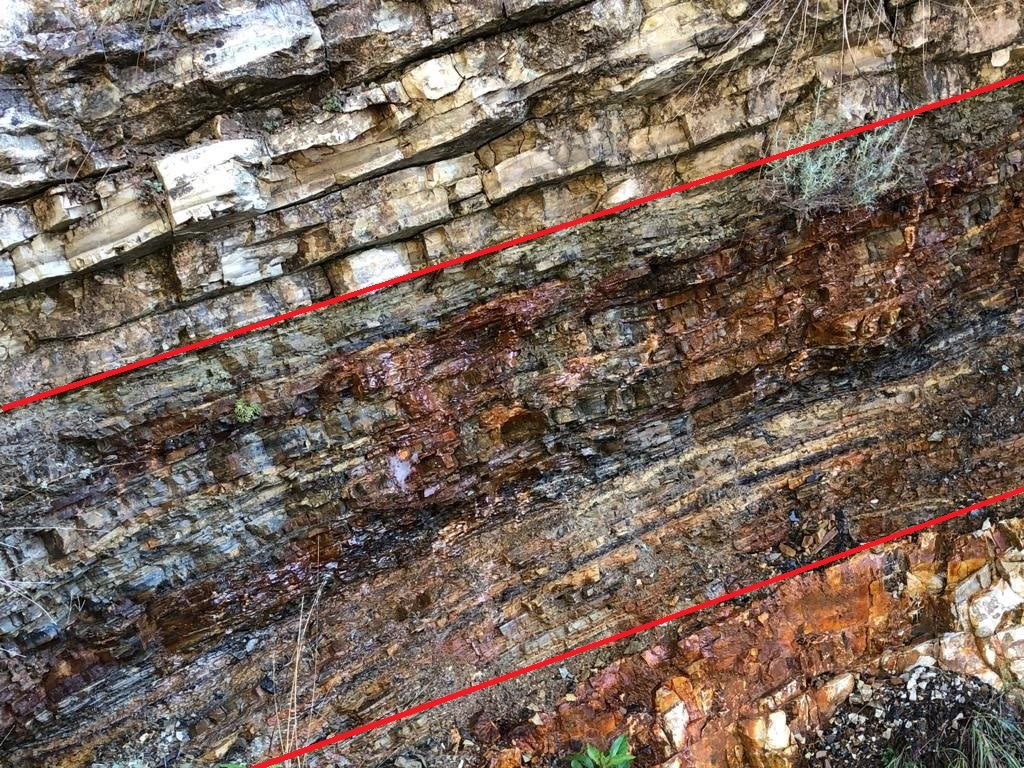
\includegraphics[width=0.66\linewidth]{images/book4/b2-19-bonarelli-level.jpg}
\par\smallskip{\small Le niveau de Bonarelli, schiste noir de l'EAO~2, entre
des calcaires clairs~; les traits rouges, tracés par le photographe, marquent
sa base et son sommet. (Picenus, CC~BY-SA~4.0, via Wikimedia Commons.)}
\end{omfigure}
% ledger: rigo24:oaes

\begin{inthefield}[Relever un événement anoxique]
Un géologue qui étudie une EAO dans une coupe de calcaires pélagiques le relève banc par banc~:
épaisseur, couleur, lamination, terriers ou leur absence, nodules de pyrite. Il échantillonne à
intervalles rapprochés et réguliers à travers l'intervalle sombre et bien au-delà, pour la teneur
en carbone organique et pour les isotopes du carbone de la matière organique et du carbonate~;
c'est le décalage des isotopes, plus que la couleur de la roche, qui permet de corréler l'événement
d'un bassin à l'autre. Parce que le schiste le plus sombre peut apparaître à des niveaux
différents selon les bassins, la courbe isotopique, et non le schiste noir, sert de repère temporel.
\end{inthefield}
% ledger: rigo24:oaes, wt24:oae2

\subsection*{Chicxulub}

La fin du Crétacé a eu une cause venue de l'extérieur. Le volume de première année a raconté comment l'iridium
de l'argile de limite a conduit à un impact, et comment la datation à l'argon a relié la limite au
cratère de Chicxulub. La structure mesure environ \qty{200}{km} de diamètre et date de \qty{66}{Ma}~; ses
roches chaudes ont alimenté une circulation d'eau pendant au moins huit millions d'années après. Les modèles
de son asymétrie souterraine désignent un impacteur venu du nord-est, incliné de 45 à \ang{60} sur
l'horizontale, à une vitesse au moins égale à la vitesse de libération de la Terre, \qty{11.2}{km.s^{-1}}, et
plus probablement d'environ \qty{20}{km.s^{-1}}. Les trapps du Deccan entraient en éruption au même moment,
avant et après l'impact~; une revue des données en 2010 a conclu que l'impact a déclenché l'extinction.
% ledger: pickersgill26:chicxulub, collins20:impact, renne:kpg, alvarez:iridium, schulte:kpg, cr03:deccan

\begin{dated}{2026}
Les âges de ce chapitre sont ceux de la Carte chronostratigraphique internationale dans sa version de juin
2026, utilisée dans toute cette série~; les enregistrements du niveau marin sont sur l'échelle de temps de 2012
de leurs fichiers, et les âges des extinctions sont ceux de Kaiho (2022). La carte est révisée au fur et à
mesure que de nouvelles datations paraissent~: vérifiez la version courante avant de citer l'âge d'une limite.
\end{dated}
% ledger: ics:base.Phanerozoic, data:b4-sealevel, kaiho22:table

\section*{Exercices}\label{sec:b2:phanerozoic-earth:exercises}

Données pour les exercices, sauf mention contraire~: \qty{111.2}{km} par degré de
latitude~; profondeur du plancher océanique $d(t) = 2500 + 350\sqrt t$ (\unit{m}, $t$
en \unit{Ma})~; aire de l'océan \qty{362}{\mega km^2}~; aire du plancher océanique
\qty{293}{\mega km^2}~; masse volumique du manteau \qty{3300}{kg.m^{-3}}~; eau de mer
\qty{1025}{kg.m^{-3}}~; masse de l'atmosphère \qty{5.1e18}{kg}, masses molaires de
l'air et du dioxyde de carbone \qty{28.97}{g.mol^{-1}} et \qty{44.01}{g.mol^{-1}}.
% ledger: earth:Rmean, ps77:depth-age, charette:ocean-volume, data:b4-ridge, katz03:thermo, noaa:seawater-1025, earth:Matm, earth:Mmol, ciaaw:abridged-2024

\begin{exercise}[$\star$]\label{exo:b2:phanerozoic-earth:1}
Dans le modèle des cartes, Le Cap se trouvait à \ang{61.9}~S il y a \qty{300}{Ma} et New York à
\ang{3.6}~S~; aujourd'hui elles se trouvent à \ang{33.9}~S et \ang{40.7}~N. (a) Dire laquelle des
quatre villes se trouvait à moins de \ang{30} de l'équateur il y a \qty{300}{Ma} (Paris à
\ang{5.1}~N, Sydney à \ang{59.5}~S). (b) Calculer, en kilomètres, le déplacement vers le nord du Cap
et de New York depuis cette époque. (c) En déduire les vitesses moyennes, en centimètres par an.
\end{exercise}
% ledger: data:b4-palaeopos, geonames4:cities

\begin{exercise}[$\star$]\label{exo:b2:phanerozoic-earth:2}
Les big five ont eu lieu à 444, 372, 251.9, 201.4 et \qty{66}{Ma}. (a) Trouver les intervalles entre crises
successives et leur moyenne. (b) À partir des âges moyens des grandes provinces ignées --- Emeishan 259,
Sibérie 250, CAMP 201, Karoo--Ferrar 183, Deccan \qty{65.5}{Ma} --- indiquer lesquelles des cinq crises se
situent à moins de \qty{2}{Ma} d'une province. (c) Un intervalle moyen rend-il les crises périodiques~?
\end{exercise}
% ledger: kaiho22:table, cr03:table

\begin{exercise}[$\star$]\label{exo:b2:phanerozoic-earth:3}
La craie de Monument Rocks s'est déposée à environ \qty{0.036}{mm} par an. (a) Calculer le temps qu'a mis une épaisseur
de \qty{91}{m}. (b) Calculer combien de fois plus vite la mer monte aujourd'hui, à \qty{3.7}{mm} par an. (c)
Expliquer pourquoi un fond marin peut recueillir une pluie de sédiments aussi lente sans être enseveli sous la vase.
\end{exercise}
% ledger: kgs:monument-rocks, ipcc:sea-level-obs

\begin{exercise}[$\star$]\label{exo:b2:phanerozoic-earth:4}
Dans une falaise, de bas en haut~: grès fluviatile à racines, sable de plage à coquilles, vase grise
du large, craie~; la craie est ensuite recouverte de nouveau par du sable de plage. (a) Repérer
où la coupe enregistre une \omterm{def:b2:phanerozoic-earth:transgression}{transgression marine}, et où une régression. (b) Dire si la transgression
prouve que le niveau marin global a monté. (c) Indiquer ce qui la rendrait plus convaincante.
\end{exercise}

\begin{exercise}[$\star\star$]\label{exo:b2:phanerozoic-earth:5}
Sur la courbe à long terme de Haq et al., le niveau marin se tenait à \qty{233}{m} au-dessus
d'aujourd'hui à \qty{97}{Ma}. (a) Calculer la vitesse moyenne de baisse depuis lors, en mètres par
million d'années puis en micromètres par an. (b) Comparer avec la hausse actuelle de \qty{3.7}{mm}
par an. (c) La courbe de New Jersey, corrigée de l'affaissement, donne environ \qty{70}{m}
à la même époque. Dire laquelle des deux courbes on retiendrait pour l'amplitude, et pourquoi.
\end{exercise}
% ledger: data:b4-sealevel, ipcc:sea-level-obs, miller05:abstract, miller20:epr

\begin{exercise}[$\star\star$]\label{exo:b2:phanerozoic-earth:6}
Une seule pulsation de la CAMP, soit environ \qty{e5}{km^3} de basalte de masse volumique
\qty{2900}{kg.m^{-3}}, est entrée en éruption en environ 500 ans. (a) Avec \qty{0.75}{\percent} de
dioxyde de carbone en masse, calculer ce qu'elle a libéré, en kilogrammes puis en moles. (b) Calculer
la masse de dioxyde de carbone que contenait l'air à \qty{278}{ppm} de 1750. (c) Comparer.
(d) Dire combien de telles atmosphères aurait fournies la province entière, soit \qty{e5}{Gt}.
\end{exercise}
% ledger: capriolo20:camp-co2, ipcc:erf-2xco2, earth:Matm, earth:Mmol, ciaaw:abridged-2024

\begin{exercise}[$\star\star$]\label{exo:b2:phanerozoic-earth:7}
Modéliser l'impacteur de Chicxulub comme une sphère de \qty{10}{km} de diamètre, de masse volumique
\qty{2630}{kg.m^{-3}}. (a) Calculer sa masse. (b) Calculer son énergie cinétique à la vitesse minimale
possible, \qty{11.2}{km.s^{-1}}, puis à \qty{20}{km.s^{-1}}. (c) La Terre perd \qty{47}{TW} de chaleur
interne par sa surface. Calculer combien d'années de cette perte représente chacune de ces énergies.
\end{exercise}
% ledger: alvarez:iridium, collins20:impact, b2dd10:half-space

\begin{exercise}[$\star\star$]\label{exo:b2:phanerozoic-earth:8}
(a) Énumérer les caractères par lesquels un schiste noir témoigne d'un \omterm{def:b2:phanerozoic-earth:oae}{événement anoxique océanique}. (b) Associer
chaque événement à une province d'âge presque identique~: Toarcien précoce, \qty{183}{Ma}~; EAO~1a, \qty{120}{Ma}~;
sachant que les basaltes du Karoo--Ferrar ont \qty{183}{Ma} et le plateau d'Ontong Java \qty{122}{Ma}. (c)
Expliquer pourquoi une simple coïncidence d'âges ne suffit pas à prouver qu'une province a causé un événement.
\end{exercise}
% ledger: rigo24:oaes, cr03:table

\begin{exercise}[$\star\star$]\label{exo:b2:phanerozoic-earth:9}
Dans le modèle, Paris se trouvait à \ang{60.9}~S il y a \qty{500}{Ma} et à \ang{5.1}~N il y
a \qty{300}{Ma}. (a) Calculer son déplacement vers le nord en degrés puis en kilomètres, et
la vitesse moyenne en centimètres par an. (b) Comparer avec la vitesse depuis \qty{300}{Ma}
(\cref{ex:b2:phanerozoic-earth:paris}). (c) Expliquer pourquoi cette vitesse est un minimum.
\end{exercise}
% ledger: data:b4-palaeopos

\begin{exercise}[$\star\star\star$]\label{exo:b2:phanerozoic-earth:10}
Supposer à la place que l'aire du plancher décroît linéairement avec l'âge, depuis un maximum à l'âge 0 jusqu'à zéro
à l'âge $T$. (a) Montrer que l'âge moyen vaut $T/3$ et que la moyenne de $\sqrt t$ vaut
$\tfrac{8}{15}\sqrt T$. (b) Avec un âge moyen de \qty{64.2}{Ma}, trouver $T$ et la profondeur moyenne. (c)
Trouver la baisse de la profondeur moyenne lorsque la vitesse d'expansion double, et la comparer avec les
\qty{774}{m} du modèle réparti. (d) Montrer que dans les deux modèles la baisse est voisine de $0.93\,c\sqrt{\bar
t}\,(1 - f^{-1/2})$, avec $\bar t$ l'âge moyen.
\end{exercise}

\begin{exercise}[$\star\star\star$]\label{exo:b2:phanerozoic-earth:11}
(a) À partir de la \cref{prop:b2:phanerozoic-earth:ridge}, montrer que $\Delta s(f) = \Delta s(2)\,(1 -
f^{-1/2})/(1 - 2^{-1/2})$. (b) Avec $\Delta s(2) = \qty{432}{m}$, trouver l'intervalle de $f$ qui
donne le maximum du Crétacé, de 50 à \qty{150}{m}. (c) Dire ce que donnerait une vitesse d'expansion ralentie à 0.8 de
celle d'aujourd'hui. (d) Expliquer pourquoi un niveau marin à long terme fixé par les dorsales est un signal lent, quel que soit le changement de
vitesse.
\end{exercise}
% ledger: data:b4-ridge, miller05:abstract

\begin{exercise}[$\star\star\star$]\label{exo:b2:phanerozoic-earth:12}
Supposer que les espèces disparaissent à taux constant, de sorte que la fraction d'une cohorte qui survit pendant
un temps $t$ vaut $2^{-t/m}$, avec une longévité médiane des espèces $m = \qty{2}{Ma}$. (a) Calculer la
fraction d'une cohorte disparue après \qty{7.4}{Ma}, durée moyenne d'un étage dans l'analyse de 1982. (b) Calculer
le temps que mettrait l'extinction de fond pour éliminer \qty{81}{\percent} des espèces. (c) La crise de la fin
du Permien a duré environ \qty{60}{ka}~: dire de combien elle a été plus rapide. (d) Expliquer pourquoi une
résolution temporelle grossière brouille la différence entre une extinction de masse et une extinction de fond.
\end{exercise}
% ledger: marshall23:resolution, stanley16:permian, burgess:end-permian

\begin{problem}[{Problème du week-end --- Quand les dorsales allaient vite}]\label{pb:b2:phanerozoic-earth:1}
Ce problème demande de combien monterait la mer, et quelle surface de terre elle submergerait, si les
dorsales s'écartaient deux fois plus vite. Utiliser les données des exercices~; l'âge moyen du plancher
océanique est de \qty{64.2}{Ma}, les dorsales ont une longueur totale de \qty{65000}{km}, l'océan actuel
contient \qty{1.33e9}{km^3} et les terres couvrent \qty{148}{\mega km^2}. Le tableau donne le pourcentage
des terres actuelles situées sous $h$ au-dessus du niveau de la mer, d'après la grille ETOPO1 à un degré.
\begin{center}
\small
\begin{tabular}{lcccccc}
\hline
$h$ (\unit{m}) & 0 & 100 & 200 & 300 & 400 & 500 \\
terres sous $h$ (\unit{\percent}) & 0 & 14.9 & 28.2 & 38.7 & 48.1 & 55.8 \\
\hline
\end{tabular}
\end{center}
Supposer, comme dans la \cref{prop:b2:phanerozoic-earth:ridge}, que chaque âge du
plancher compris entre 0 et l'âge $\tau$ auquel il est subduit couvre la même aire.

\noindent\textbf{Partie I --- Le plancher océanique aujourd'hui.}
\begin{enumerate}
  \item Trouver la profondeur du plancher aux âges 0, 25, 64.2 et \qty{100}{Ma}.
  \item Trouver $\tau$ à partir de l'âge moyen, et la profondeur du plancher le plus ancien.
\item Trouver le taux d'expansion complet moyen $u = A_{\text{f}}/(L\tau)$, en kilomètres
par million d'années et en millimètres par an. Dire s'il est lent, intermédiaire ou rapide.
\item Montrer que la profondeur moyenne du plancher vaut
$2500 + \tfrac23 \times 350\sqrt\tau$, et la calculer.
\item La profondeur moyenne mesurée du plancher daté est de \qty{4265}{m}.
Donner deux raisons pour lesquelles le modèle est plus profond.
\item Calculer le volume d'eau qui reposerait au-dessus du plancher
dans le modèle, et le comparer au volume de l'océan entier.
\end{enumerate}

\noindent\textbf{Partie II --- Une dorsale en coupe.}
\begin{enumerate}[resume]
\item Calculer la demi-vitesse d'expansion $v$, à \qty{0.1}{km.Ma^{-1}}
près, et la largeur de plancher de chaque côté de la dorsale.
  \item Calculer la profondeur du plancher à \qty{1000}{km} de l'axe.
\item Montrer que la section de la dorsale au-dessus de la profondeur
du plancher le plus ancien, en comptant les deux flancs, a pour
aire $\tfrac23 v c\,\tau^{3/2}$, et la calculer en kilomètres carrés.
  \item Calculer le volume de l'ensemble du système de dorsales au-dessus de cette profondeur.
  \item Indiquer quelle fraction du volume de l'océan cela représente.
  \item Expliquer pourquoi une dorsale qui s'étend plus vite se tient plus haut en moyenne.
\end{enumerate}

\noindent\textbf{Partie III --- Deux fois plus vite.}
\begin{enumerate}[resume]
\item La vitesse d'expansion double, à aire de plancher et longueur de dorsale
inchangées. Calculer le nouveau $\tau$ et la nouvelle profondeur moyenne.
  \item Calculer de combien la profondeur moyenne diminue.
  \item Calculer le volume d'eau que le plancher chasse hors des bassins.
  \item Calculer de combien cette eau élèverait la mer si elle était répartie sur l'océan actuel.
  \item Tenir compte de l'affaissement du plancher sous l'eau supplémentaire pour trouver la hausse $\Delta s$.
\item Le maximum à long terme du Crétacé était d'environ \qty{100}{m}.
Calculer l'augmentation de la vitesse d'expansion qui donnerait ce niveau.
\end{enumerate}

\noindent\textbf{Partie IV --- La mer au-dessus des terres.}
\begin{enumerate}[resume]
  \item Calculer l'aire de terre que submergerait une hausse de \qty{100}{m}.
  \item Calculer, par interpolation dans le tableau, l'aire que submergerait une hausse de \qty{432}{m}.
  \item Expliquer pourquoi la mer doit monter de moins de \qty{432}{m} une fois qu'elle s'étend sur les terres.
\item Calculer le volume nécessaire pour élever la mer par paliers de
\qty{100}{m} jusqu'à \qty{400}{m}, en moyennant l'aire submergée sur chaque
palier (\cref{prop:b2:phanerozoic-earth:flooding}). Le volume à placer est
$\qty{0.432}{km} \times \qty{362}{\mega km^2}$. Indiquer où s'arrête la mer.
  \item Calculer quelle part des terres actuelles elle couvre alors, en pourcentage.
  \item En résumé, dire de combien le doublement de la vitesse d'expansion élèverait la mer dans ce modèle.
\end{enumerate}
\end{problem}
% ledger: ps77:depth-age, seton:mean-age, seton:rate-classes, noaa:ridge, charette:ocean-volume, data:b4-ridge, data:b4-floor-depth, katz03:thermo, noaa:seawater-1025, data:b4-hyps, miller05:abstract
